\begin{frame}
    \autotitle
    \begin{center}
        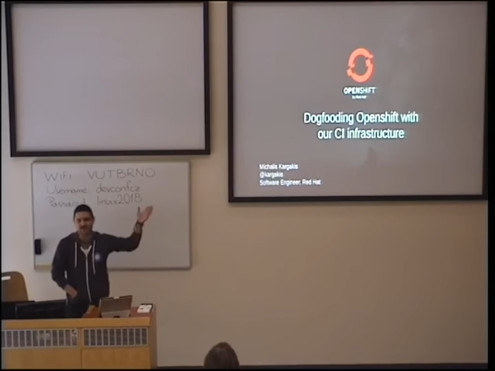
\includegraphics[scale=.4]{img/pres_2018.jpg} \\
        \textit{Dogfooding Openshift with our CI infrastructure}, \\
        Michalis Kargakis (2018-01-27) \\
        \url{https://www.youtube.com/watch?v=rLLEjodflYw}
    \end{center}
    \note{
        Continuing with the historical theme, but moving on to motivation, there
        is a presentation by Michalis which was posted in our chat recently.  It
        is contemporaneous --- n.b.: four days before the beginning of the
        \texttt{ci-operator} repository/history --- and goes through many of the
        problems the CI system at the time had.
    }
\end{frame}

\subsection{Past}

\begin{frame}
    \autotitle
    \begin{itemize}
        \item
            Jenkins \only<2>{(R.I.P.)}
            \begin{itemize}
                \item<2> Ruby (OpenShift v2), Python, Bash, \ldots
                \item<2> \emph{slow}
                \item<2> unmaintained
                \item<2> \emph{unmaintainable}
            \end{itemize}
        \item<2>
            Kubernetes
            \begin{itemize}
                \item \url{https://github.com/kubernetes/test-infra.git}
                \item Prow
            \end{itemize}
        \item<2>
            OpenShift
            \begin{itemize}
                \item \texttt{ImageStream}s
                \item \texttt{Build}s
                \item multi-tenancy
                \item \ldots
            \end{itemize}
    \end{itemize}
    \note{
        They can be summarized mostly with one word.

        The CI "system" was a mixture of Ruby (as was OpenShift v2), Python, and
        Bash scripts, used a very inefficient model on top of that, and was
        mostly unmaintained and unmaintainable.

        Meanwhile, Kubernetes (our upstream project) had \texttt{test-infra} and
        Prow: a CI system which used the platform itself and a language and
        concepts that were familiar to OpenShift developers.

        OpenShift also had many unique features which could be used to extend
        the upstream system (at the time, many were later contributed upstream,
        although a unique set still remains).

        So we decided to adopt Prow and integrate it into our product.
    }
\end{frame}

\subsection{Prow}

\begin{frame}[fragile]
    \autotitle
    \footnotesize
    \url{https://github.com/kubernetes/test-infra/blob/master/prow/life_of_a_prow_job.md}
    \scriptsize
    \begin{verbatim}
apiVersion: prow.k8s.io/v1
kind: ProwJob
metadata:
  name: 32456927-35d9-11e7-8d95-0a580a6c1504
spec:
  job: pull-test-infra-bazel
  decorate: true
  pod_spec:
    containers:
    - image: gcr.io/k8s-staging-test-infra/bazelbuild:latest-test-infra
  refs:
    base_ref: master
    base_sha: 064678510782db5b382df478bb374aaa32e577ea
    org: kubernetes
    pulls:
    - author: ixdy
      number: 2716
      sha: dc32ccc9ea3672ccc523b7cbaa8b00360b4183cd
    repo: test-infra
  type: presubmit
    \end{verbatim}
    \note{
        In Prow, the unit of work is the \texttt{ProwJob}: a native Kubernetes
        object which links the information from the repository (repository,
        revision, pull request, etc.) to the work that must be done in the build
        cluster (in the form of a \texttt{Pod} spec).
    }
\end{frame}

\begin{frame}[fragile]
    \autotitle
    \scriptsize
    \url{https://github.com/openshift/release/blob/master/ci-operator/jobs/openshift/ci-tools/openshift-ci-tools-master-presubmits.yaml}
    \begin{verbatim}
presubmits:
  openshift/ci-tools:
  - branches:
    - ^master$
    - ^master-
    cluster: build04
    labels:
      ci.openshift.io/generator: prowgen
      pj-rehearse.openshift.io/can-be-rehearsed: "true"
    name: pull-ci-openshift-ci-tools-master-unit
    spec:
      containers:
      - args:
        - --gcs-upload-secret=/secrets/gcs/service-account.json
        - --image-import-pull-secret=/etc/pull-secret/.dockerconfigjson
        - --report-credentials-file=/etc/report/credentials
        - --target=unit
        command:
        - ci-operator
        image: ci-operator:latest
    \end{verbatim} %$
    \note{
        A Prow job has to be registered before it can be executed.  We do that
        using files under \texttt{ci-operator/jobs} in the
        \texttt{openshift/release} repository.  Note that this is extremely
        anachronistic, almost nothing shown here existed at the time:
        \begin{itemize}
            \setlength\itemsep{-0.25em}
            \item there was only a single cluster
            \item there was no \texttt{prowgen}
            \item there was no \texttt{rehearse}
            \item artifact upload was done differently
            \item images were not imported from other clusters
            \item there was no results server
        \end{itemize}
        However, we do not want every user to have to build their CI pipeline
        from zero…
    }
\end{frame}

\begin{frame}[fragile]
    \autotitle
    \footnotesize
    \url{https://github.com/openshift/release/blob/master/ci-operator/config/openshift/ci-tools/openshift-ci-tools-master.yaml}
    \scriptsize
    \begin{multicols}{2}
    \begin{verbatim}
base_images:
  os:
    name: centos
    namespace: origin
    tag: stream8
binary_build_commands: >
  make production-install
build_root:
  from_repository: true
  use_build_cache: true
images:
- context_dir: >
    images/ci-operator/
  from: os
  inputs:
    bin:
      paths:
      - destination_dir: .
        source_path: >
          /go/bin/ci-operator
  to: ci-operator
  \end{verbatim}
  \columnbreak
  \begin{verbatim}
promotion:
  namespace: ci
  tag: latest
test_binary_build_commands: >
  make race-install
tests:
- as: unit
  commands: make test
  container:
    from: src
- as: e2e
  steps:
    test:
    - as: e2e
      commands: make e2e
      from: test-bin
    \end{verbatim} %$
    \end{multicols}
    \note{
        The \texttt{ci-operator} configuration file is a standard description of
        the CI pipe\-line for a given repository.  This is the configuration
        used in \texttt{ci-tools}.  It simpler because we are not an OpenShift
        component, but otherwise demonstrates the major concepts:
        \begin{itemize}
            \item input images
            \item image builds
            \item unit/E2E tests
            \item image promotion
        \end{itemize}
    }
\end{frame}
